\documentclass[twocolumn]{article}
\usepackage{hyperref}
\usepackage{settings}
\usepackage{graphicx}
\renewcommand{\tablename}{Tabela}
\renewcommand{\figurename}{Figura}
\begin{document}

\title{Descritores musicais e audiência no YouTube: uma exploração de faixas rotuladas Hard Rock}

\author{Felipe Cunha(felipe.cunha@estudante.ufjf.br)}
\author{Marcelo Machado (marcelo.machado@ufjf.br)}

\maketitle

\section*{Introdução}
Descritores de áudio representam propriedades musicais \cite{schedl2014mir}, cuja relação com sucesso já foi investigada em rankings como o Billboard Hot 100 \cite{askin2017popular}. Aqui, descrevem-se energia, dançabilidade e acusticidade de faixas rotuladas Hard Rock associadas a vídeos de menor e maior audiência no YouTube. O objetivo é comparar distribuições e gerar hipóteses para estudos independentes. Visualizações medem audiência do vídeo, sem representar todos os ouvintes da canção.

\section*{Método}
Utilizaram-se o snapshot \textit{Spotify and Youtube}, de Rastelli, com coleta declarada em 07/02/2023, e o rótulo exato \textit{hard-rock} do Spotify Tracks Dataset, de Pandya. A interseção por ID contém 176 faixas. Após filtros de marca oficial do publicador, unicidade, contagem válida e datas de catálogo, a janela 1980--1989 contém 47 faixas de 20 artistas. As datas de catálogo não foram comprovadas como primeiros lançamentos.

Antes de inspecionar descritores, selecionou-se uma faixa por artista por hash fixo. Os 20 candidatos foram divididos pela mediana de suas visualizações: menor audiência abaixo de 89.776.313,5; maior, igual/acima. IDs e corte permaneceram fixos após perdas, sem reposição. Compararam-se os três descritores da edição Spotify, em escala [0,1], por pontos individuais, mediana e intervalo interquartil (IIQ).

O autor relatou escuta dos 20 pares, sem identificação técnica de master. Intros e finais narrativos foram aceitos quando a gravação-base correspondia. Após uma prévia técnica, excluíram-se conservadoramente dois pares com extensão musical de encerramento e um ID original não suficientemente confirmado, cuja alternativa estava ausente dos snapshots. Restaram 17 faixas com os três descritores válidos.

\section*{Resultados}
Incluíram-se sete das dez faixas do grupo menor e as dez do maior; as três perdas ocorreram no primeiro. Na Figura~\ref{fig:descritores}, o grupo maior apresenta medianas menores de energia (0,7545 versus 0,9310) e dançabilidade (0,3505 versus 0,5400). As medianas de acusticidade são próximas (0,02595 versus 0,02020), sem demonstração de equivalência. Os intervalos dos valores individuais se sobrepõem nos três descritores, indicando heterogeneidade dentro dos grupos.

\begin{figure}[ht]
\centering
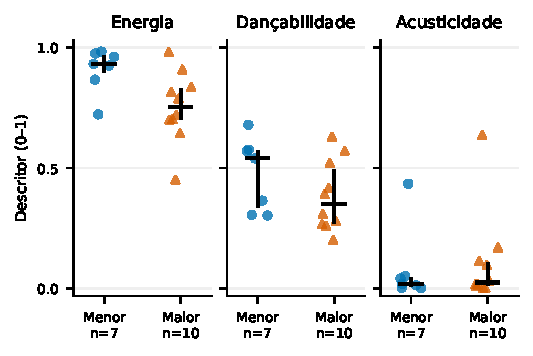
\includegraphics[width=\columnwidth]{figures/hard-rock-validated-paper.pdf}
\caption{Distribuições por audiência histórica: círculos azuis, menor ($n=7$); triângulos laranja, maior ($n=10$). Traço horizontal: mediana; vertical: IIQ. Cada ponto representa uma faixa de artista distinto.}
\label{fig:descritores}
\end{figure}

\section*{Discussão e limites}
O achado sugere, como hipótese \textit{pós-hoc}, que medianas menores de energia e dançabilidade possam acompanhar maior audiência em outro conjunto comparável. Testá-la exige novas gravações, critérios prévios e consideração da idade do vídeo, formato, artista e subestilo. Os mesmos dados que sugeriram essa hipótese não a confirmam.

As perdas no grupo menor podem modificar seu perfil. O ano mediano de catálogo é 1984 em ambos, mas faltam as datas de publicação dos 17 vídeos, impedindo avaliar exposição; o formato é desconhecido em 12 casos. A interseção e o rótulo catalográfico restringem conclusões; remasters não comprovam master idêntico. Não houve amostragem representativa, teste de significância ou avaliação causal/preditiva.

\section*{Conclusão}
A contribuição é uma descrição rastreável de 17 pares e uma hipótese para avaliação independente. As diferenças de medianas observadas coexistem com sobreposição e limitações de cobertura e exposição, sem estabelecer uma fórmula do sucesso.

\bibliographystyle{abntex2-alf}
\bibliography{references}

\end{document}
